%%%%%%%%%%%%%%%%%%%%%%%%%%%%%%%%%%%%%%%%%%%%%%%%%%%%%%%%%%%%%%%%%%%%%%%%%%
%% Review Volume (last updated on 2014/03/05) %%
%% Trim Size: 9.61in x 6.69in %%
%% Text Area: 8in (include runningheads) x 5in %%
%% Main Text: 10 on 13pt %%
%% For support: Yolande Koh, <ykoh@wspc.com.sg> %%
%% D. Rajesh Babu, <rajesh@wspc.com.sg> %%
%%%%%%%%%%%%%%%%%%%%%%%%%%%%%%%%%%%%%%%%%%%%%%%%%%%%%%%%%%%%%%%%%%%%%%%%%%
%%
%\documentclass[wsdraft]{ws-rv961x669} % to draw border line around text area
%\documentclass{ws-rv961x669}
\documentclass[addchapnum]{ws-rv961x669} % to add chapter number in volume
\usepackage{ws-rv-van} % numbered citation/references (default)
%\usepackage{ws-rv-thm} % comment this line when `amsthm / theorem / ntheorem` package is used
%\usepackage{subfigure} % required only when side-by-side / subfigures are used
\usepackage{ws-index} % required only when multiple indexes are used
%\usepackage[colorlinks=false]{hyperref}
%\usepackage{doi}
\usepackage{bbm}
\usepackage{amsmath}
\usepackage{amssymb}
\makeindex
\newindex{aindx}{adx}{and}{Author Index} % author index
\renewindex{default}{idx}{ind}{Subject Index} % subject index

\newcommand{\req}[1]{Eq.~(\ref{#1})}
 
\begin{document}

\chapter[Dynamic flavor mixing through transition moments]{Dynamic flavor mixing through transition moments\label{JR_ch1}}

\author[J. Rafelski and A. Steinmetz]{Johann Rafelski and Andrew Steinmetz\footnote{JohannR@Arizona.EDU, AJSteinmetz@Arizona.EDU}}
\aindx{Rafelski, J.}
\aindx{Steinmetz, A.}

\address{Department of Physics, The University of Arizona, Tucson, AZ 85721, USA}

\begin{abstract} 
As neutrinos are naturally massless in the standard model the observed flavor oscillation presents a problem. Moreover it is unknown if neutrinos are Dirac-type or Majorana-type fermions. We show that the required neutrino flavor mixing can be driven by electromagnetic transition dipole moments. We analyze neutrino eigenstates and the sensitivity of the rotation mixing matrix to strong electromagnetic fields.
\end{abstract}

\markboth{Johann Rafelski and Andrew Steinmetz}{Neutrinos in EM fields} % Customized running heads

\body

%\tableofcontents\

%%%%%%%%%%%%%%%%%%%%%%%%%%%%%%%%%%%%
\section{Introduction}
\label{sec:intro}
%%%%%%%%%%%%%%%%%%%%%%%%%%%%%%%%%%%%

In this work we look at the connection between neutrino transition magnetic dipole moments~\cite{Shrock:1980vy,Shrock:1982sc} and neutrino flavor oscillation. Neutrinos once were the dominant form of energy density in the universe~\cite{Rafelski:2023emw} and are also important in the context of stellar evolution and supernova. There is profound interest in understanding their physical properties due to their importance as a bridge to beyond standard model (BSM) physics~\cite{DUNE:2020fgq}. It is also unknown which hierarchy neutrinos follow therefore probing the EM properties of neutrinos could contribute evidence for one model over the other. Their electromagnetic (EM) properties have been considered before~\cite{Giunti:2014ixa,Chukhnova:2019oum,Popov:2019nkr} but to best of our knowledge this is a first consideration of the full EM contribution to flavor oscillation.

Neutrinos being electrically neutral, have no intrinsic magnetic moment due to their spin, therefore any magnetic moment present is considered anomalous~\cite{Steinmetz:2018ryf}. A small anomalous magnetic moment (AMM) can be introduced into the neutrino Lagrangian via a Pauli term. Since transition AMM elements serve to break lepton number conservation allowing for $\nu_{\ell}+\gamma\rightarrow\nu_{\ell'}$ processes, neutrinos could be remixed when exposed to strong EM fields similar to remixing within matter in the Mikheyev-Smirnov-Wolfenstein (MSW) effect~\citep{Wolfenstein:1977ue,Mikheyev:1985zog}.

The size of the neutrino magnetic dipole moment is relatively small with a lower bound determined by the standard model and an upper bound from reactor or solar observations given by~\citep{Studenikin:2016ykv,Canas:2015yoa,AristizabalSierra:2021fuc}
\begin{align}
    \label{momentbound:1}
    10^{-19}\mu_{B}<\mu_{\nu}^\mathrm{eff}<10^{-10}\mu_{B}\,,\qquad\mu_{B}=\frac{e\hbar}{2m}
\end{align}
where $\mu_{B}$ is the Bohr magneton and $\mu_{\nu}^\mathrm{eff}$ is the effective and characteristic size of the neutrino magnetic moment.

Considering higher order diagrams neutrino should manifestation non-minimal EM interactions~\citep{Shrock:1980vy} of the form
\begin{align}
    \label{mu:1}
    \mu_{\ell\ell'}=
	\begin{pmatrix}
		\mu_{ee} & \mu_{e\mu} & \mu_{e\tau} \\
		\mu_{e\mu}^{*} & \mu_{\mu\mu} & \mu_{\mu\tau} \\
		\mu_{e\tau}^{*} & \mu_{\mu\tau}^{*} & \mu_{\tau\tau}
	\end{pmatrix}\,,
\end{align}
where $\ell$ are the neutral lepton flavor indices $\ell\in\nu_{e},\nu_{\mu},\nu_{\tau}$. The transition moments are generally considered small but BSM physics is capable of producing an abnormally large electromagnetic dipole~\citep{Ohlsson:2012kf,Lindner:2017uvt,Brdar:2020quo} within the bounds of~\req{momentbound:1} which may manifest itself in strong field or/and dense matter environments.

%%%%%%%%%%%%%%%%%%%%%%%%%%%%%%%%%%%%%%%
\section{Description of neutrino flavor mixing}
\label{sec:numass}
%%%%%%%%%%%%%%%%%%%%%%%%%%%%%
For clarity of presentation we recall briefly textbook level neutrino physics: Experiment shows that neutrino mass and flavor eigenstates differ. This misalignment between the two representations is described as rotation of the neutrino flavor 3-vector where $N=3$ is the number of generations. The unitary mixing matrix $V$ allows for the change of basis between mass and flavor eigenstates as 
\begin{alignat}{1}
	\label{basis:1} \nu_{\ell}=\sum_{k=1}^{3}V_{\ell k}\nu_{k}\,\rightarrow
	\begin{pmatrix}
		\nu_{e}\\
		\nu_{\mu}\\
		\nu_{\tau}
	\end{pmatrix}=
	\begin{pmatrix}
		V_{e1} & V_{e2} & V_{e3}\\
		V_{\mu1} & V_{\mu2} & V_{\mu3}\\
		V_{\tau1} & V_{\tau2} & V_{\tau3}
	\end{pmatrix}
	\begin{pmatrix}
		\nu_{1}\\
		\nu_{2}\\
		\nu_{3}
	\end{pmatrix}\,,
\end{alignat}
where $\nu_{\ell}$ is the neutrino state four-spinor written in the flavor basis while in the mass basis we use $\nu_{k}$ with $k\in1,2,3$. Hereafter we will use implied summation  over repeated indices.

The parameterization of the components of the mixing matrix depends on the Dirac- or Majorana-nature of the neutrinos. We consider $U$ to be the Dirac neutrino matrix which in the standard parameterization~\citep{Schwartz:2014sze}, can be expressed as
\begin{alignat}{1}
	\label{rotation:1} U_{\ell k} =
	  \begin{pmatrix}
		  c_{12}c_{13} & s_{12}c_{13} & s_{13}e^{-i\delta}\\
		  -s_{12}c_{23} - c_{12}s_{13}s_{23}e^{i\delta} & c_{12}c_{23} - s_{12}s_{13}s_{23}e^{i\delta} & c_{13}s_{23}\\
		  s_{12}s_{23} - c_{12}s_{13}c_{23}e^{i\delta}& -c_{12}s_{23} - s_{12}s_{13}c_{23}e^{i\delta} & c_{13}c_{23}
	  \end{pmatrix}\,,
\end{alignat}
where $c_{ij} = \mathrm{cos}(\theta_{ij})$ and $s_{ij} = \mathrm{sin}(\theta_{ij})$. In this convention, the three mixing angles $(\theta_{12}, \theta_{13}, \theta_{23})$, are understood to be the Euler angles for generalized rotations and $\delta$ is the CP-violating complex phase. 

For the Majorana case of interest to us we must allow a greater number of complex phases described by an additional matrix $P$
\begin{alignat}{1}
	\label{phases:1} &V_{\ell k} = U_{\ell k'}P_{k'k}\,,\\
	\label{phases:3} &P_{kk'} = \mathrm{diag}(e^{i\rho},e^{i\sigma},1)\,.
\end{alignat}
Majorana neutrinos allow up to two additional complex phases $\rho$ and $\sigma$ which along with $\delta$ participate in CP-violation. The mixing matrix $V$ defined in \req{phases:1} can then be used to diagonalize the mass matrix $M$ from the flavor basis into the mass basis as
\begin{align}
    \label{diag:1}
    V_{\ell k}^{T}M_{\ell\ell'}V_{\ell'k'} = M_{kk'} = \mathrm{diag}(m_{1},m_{2},m_{3})\,.
\end{align}
The masses $m_{k}$ are taken to be real and positive labelling the propagating states of the three neutrinos.

The Majorana mass term in the Lagrangian can be written in chiral flavor basis as
\begin{alignat}{1}
	\label{mass:1} -\mathcal{L}_{\mathrm{mass}}^{\mathrm{Maj.}}=\frac{1}{2}\nu_{L,\ell}^{T}C^{\dag}M_{\ell\ell'}\nu_{L,\ell'}+\mathrm{h.c}\,,\qquad
    M_{\ell\ell'}^{T}=M_{\ell\ell'}\,,
\end{alignat}
where $\nu_{L}$ refers to left-handed chiral states. We note the Majorana mass matrix is symmetric and in general complex~\cite{Adhikary:2013bma}. The charge conjugation matrix $C$ is defined in Ref.~\cite{Itzykson:1980rh}, p.692.

%%%%%%%%%%%%%%%%%%%%%%%%%%%%%%%%%%%%%%%
\section{Neutrino electromagnetic dipole moment dynamics}
\label{sec:numoment}
%%%%%%%%%%%%%%%%%%%%%%%%%%%%%%%%%%%%%%%
The electromagnetic dipole behavior of the neutrino depend on mathematical properties of the tensor product $\sigma_{\alpha\beta}F^{\alpha\beta}$ where $\sigma_{\alpha\beta}$ is the $4\times 4$ spin tensor defined by the commutator of the gamma matrices and $F^{\alpha\beta}$ is the electromagnetic field tensor. In our description, $F^{\alpha\beta}$ is the influence an externally prescribed field $A^{\alpha}_\mathrm{ext}(x)$ which imparts a force on the neutrino fields.

We prefer to work in the Weyl (chiral) spinor representation where the EM contribution is diagonal in spin space. Therefore we evaluate the product $\sigma_{\alpha\beta}F^{\alpha\beta}$ in the chiral representation following Feynman and Gell-mann\cite{Feynman:1958ty} yielding
\begin{align}
    \label{chiral:1}
    -\frac{1}{2}\sigma_{\alpha\beta}F^{\alpha\beta}=
    \begin{pmatrix}
        \vec{\sigma}\cdot(\vec{B}+i\vec{E}/c) & 0\\
        0 & \vec{\sigma}\cdot(\vec{B}-i\vec{E}/c)
    \end{pmatrix}\equiv
    \begin{pmatrix}
        \vec{\sigma}\cdot\vec{f}_{+} & 0 \\
        0 & \vec{\sigma}\cdot\vec{f}_{-}
    \end{pmatrix}\,,
\end{align}
where we have defined the complex electromagnetic field $\vec{f}_{\pm}=\vec{B}\pm i\vec{E}/c$.

For later convenience we note how the EM invariants $\mathcal{S}$ and $\mathcal{P}$ can help understand the AMM term 
\begin{gather}
    \left(\frac{1}{2}\sigma_{\alpha\beta}F^{\alpha\beta}\right)^{2}=
    \begin{pmatrix}
        \mathcal{S}+i\mathcal{P} & 0\\
        0 & \mathcal{S}-i\mathcal{P}
    \end{pmatrix}\,,\\
    \mathcal{S}\equiv\frac{1}{2}\left(B^{2}-E^{2}/c^{2}\right)\,,\qquad
    \mathcal{P}\equiv\vec{B}\cdot\vec{E}/c\,,\qquad
    \frac{1}{2}\vec{f}_{\pm}\cdot\vec{f}_{\pm}=\mathcal{S}\pm i\mathcal{P}\,.
\end{gather}
Moreover, for the product of $\vec{f}_{\pm}$ with its complex conjugate we find
\begin{align}
        \label{cross:1}
        \frac{1}{2}\left(\vec{\sigma}\cdot\vec{f}_{\pm}\right)\left(\vec{\sigma}\cdot\vec{f}_{\mp}\right)=T^{00}\mp \sigma_{i}T^{0i}\,,
\end{align}
where we recognize the  stress-energy tensor $T^{\alpha\beta}$ components $T^{00}$ and $T^{0i}$ respectively
\begin{align}
    T^{00}=\frac{1}{2}\left(B^{2}+E^{2}/c^{2}\right)\,,\qquad
    T^{0i}=\frac{1}{c}\varepsilon_{ijk}E_{j}B_{k}\,.
\end{align}
Using the identity in \req{chiral:1} and \req{cross:1} we also find the interesting relationship
\begin{align}
    \label{cross:2}
    \frac{1}{2}\left(\sigma_{\alpha\beta}F^{\alpha\beta}\right)\left(\sigma_{\alpha\beta}F^{\alpha\beta}\right)^{\dag}=
    -\gamma_{\alpha}\left(C^{\dag}\gamma_{\beta}C\right)T^{\alpha\beta}\,.
\end{align}

Now that we have elaborated on the relevant EM field identities, we turn to the magnetic dipole. The effective Majorana AMM Pauli Lagrangian in the flavor basis is given by~\cite{Shrock:1980vy}
\begin{align}
	\label{moment:1} -\mathcal{L}_{\mathrm{AMM}}^\mathrm{Maj.}=\frac{1}{2}\nu_{L,\ell}^{T}C^{\dag}\left(\mu_{\ell\ell'}\frac{1}{2}\sigma_{\alpha\beta}F^{\alpha\beta}\right)\nu_{L,\ell'}+\mathrm{h.c.}
\end{align}
The left-handed spinors $\nu_{L}$ are still four component. The magnetic moment matrix acts in flavor space, see \req{mu:1}, and it satisfies for CPT reasons the following constraints~\cite{Giunti:2014ixa}
\begin{alignat}{1}
	\label{props:1}
    \mu_{\ell\ell'}^{\dag}=\mu_{\ell\ell'}\,,\qquad
    \mu_{\ell\ell'}^{T}=-\mu_{\ell\ell'}\,,
\end{alignat}
{\it i.e.\/} the AMM matrix $\mu$ is Hermitian and fully anti-symmetric. This requires that the transitional magnetic moment elements are purely imaginary while all diagonal AMM matrix elements vanish.

We can combine the AMM contribution and the mass term in~\req{mass:1} and~\req{moment:1} to write an effective Lagrangian containing both
\begin{align}
	\label{massmom:1}
    \mathcal{L}_\mathrm{eff}^\mathrm{Maj.} =
    \mathcal{L}_\mathrm{mass}^\mathrm{Maj.} + \mathcal{L}_\mathrm{AMM}^\mathrm{Maj.} = 
    -\frac{1}{2}\nu_{L,\ell}^{T}C^{\dag}\left(M_{\ell\ell'}+\mu_{\ell\ell'}\frac{1}{2}\sigma_{\alpha\beta}F^{\alpha\beta}\right)\nu_{L,\ell'}+\mathrm{h.c.}
\end{align}
We define the generalized mass-dipole matrix $\mathcal{M}_{\ell\ell'}$ present in \req{massmom:1} as
\begin{align}
	\label{massmom:2}
    \mathcal{M}_{\ell\ell'}(E,B)\equiv M_{\ell\ell'}+\mu_{\ell\ell'}\frac{1}{2}\sigma_{\alpha\beta}F^{\alpha\beta}\,.
\end{align}

As neutrinos must propagate as energy eigenstates, it is the diagonalization of the Hermitian product $\mathcal{M}\mathcal{M}^{\dag}$ of \req{massmom:2} rather than \req{diag:1} which must be accomplished. If one uses the original rotation matrix defined in \req{phases:1}, the result will still possess off-diagonal terms. These electromagnetic components then facilitate time-dependant oscillation among the free-particle mass eigenstates~\cite{Giunti:2014ixa}. We seek to then describe a modified rotation which places the neutrinos into their true propagating energy eigenstates.

%%%%%%%%%%%%%%%%%%%%%%%%%%%%%%%%%%%%%%%
\section{Toy model: Magnetic-flavor mixing for two generations}
\label{sec:mix}
%%%%%%%%%%%%%%%%%%%%%%%%%%%%%%%%%%%%%%%
Considering experimental data on neutrino oscillations, it is understood that either the two heavier (normal hierarchy) or the two lighter (inverted hierarchy) neutrino states are close together in mass. If the electromagnetic properties of the neutrino do indeed lead to flavor mixing effects, then it is likely the closer pair of neutrino mass states that are most sensitive to effective potentials phenomenon. In the spirit of Bethe~\cite{Bethe:1986ej}, we therefore explore the $N=2$ two generation $(\nu_{e},\nu_{\mu})$ model.

Following the properties established in \req{props:1} and \req{massmom:2} we write down the two generation mass and dipole matrices as
\begin{alignat}{1}
	\label{mix:1} M_{\ell\ell'}= 
	\begin{pmatrix}
		m_{\nu_{e}} & {\delta m}\\
		{\delta m} & m_{\nu_{\mu}}
	\end{pmatrix}\,,\qquad
	\mu_{\ell\ell'} = 
	\begin{pmatrix}
		0 & i\delta\mu\\
		-i\delta\mu & 0
	\end{pmatrix}\,.
\end{alignat}
The AMM coupling $\delta\mu$ is taken to be real with a pure imaginary coefficient. While the mass elements $m_{\nu_{e}}$, $m_{\nu_{\mu}}$, and ${\delta m}$ are generally complex, we will for illustration take them to be fully real
\begin{align}
    m_{\nu_{e}}=m_{\nu_{e}}^{*}\,,\qquad
    m_{\nu_{\mu}}=m_{\nu_{\mu}}^{*}\,,\qquad
    \delta m^{*}=\delta m\,,
\end{align}
making the mass matrix $M$ Hermitian. This allows an easier evaluate the EM contribution to mixing rather than complications from the mass matrix.

Using \req{mix:1}, we write the mass-dipole matrix in \req{massmom:2} in terms of spin-flavor components as
\begin{align}
	\label{mix:2}
    \mathcal{M}_{\ell\ell'} = 
	\begin{pmatrix}
		m_{\nu_{e}} & {\delta m}+i\delta\mu\sigma_{\alpha\beta}F^{\alpha\beta}/2\\
		{\delta m}-i\delta\mu\sigma_{\alpha\beta}F^{\alpha\beta}/2 & m_{\nu_{\mu}}
	\end{pmatrix}\,.
\end{align}
In terms of \req{mix:1}, we can write the Hermitian mass-dipole square $\mathcal{M}\mathcal{M}^{\dag}$ as
\begin{align}
    \label{herm:1}
    \begin{split}
        (\mathcal{M}\mathcal{M}^{\dag})_{\ell\ell'}
        &=(MM^{\dag})_{\ell\ell'}+A_{\ell\ell'}+(\mu\mu^{\dag})_{\ell\ell'}\frac{1}{4}\left(\sigma_{\alpha\beta}F^{\alpha\beta}\right)\left(\sigma_{\alpha\beta}F^{\alpha\beta}\right)^{\dag}\\
        &+(M\mu^{\dag})_{\ell\ell'}\frac{1}{2}\left(\sigma_{\alpha\beta}F^{\alpha\beta}\right)^{\dag}
        +(\mu M^{\dag})_{\ell\ell'}\frac{1}{2}\left(\sigma_{\alpha\beta}F^{\alpha\beta}\right)\,,        
    \end{split}
\end{align}
where we have also included the linear term for matter weak interactions~\cite{Wolfenstein:1977ue} given by
\begin{align}
    \label{matter:1}
    A_{\ell\ell'}=A
    \begin{pmatrix}
        1 & 0\\
        0 & 0
    \end{pmatrix}\,,\qquad
    A\propto G\rho_{e}\,.
\end{align}
The coefficient $G$ is the Fermi constant and $\rho_{e}$ is the density of electron matter that the neutrinos are propagating through. \req{herm:1} can be simplified somewhat further by recalling that $M^{\dag}=M$ and $\mu^{\dag}=\mu$.

According to \req{diag:1}, the mass matrix in \req{mix:1} can be diagonalized by the unitary matrix $V$ which in the two generation case is given by a Cabibbo-style rotation matrix
\begin{align}
    \label{rot:1}
    V_{\ell k}=
    \begin{pmatrix}
        \cos\theta & \sin\theta\\
        -\sin\theta & \cos\theta
    \end{pmatrix}\,.
\end{align}
For a real Hermitian $2\times 2$ mass matrix, the rotation matrix $V$ only depends on the angle $\theta$. We note that because the transition magnetic moment matrix $\mu$ commutes with the mixing matrix $V$ we can write the following relations
\begin{align}
    V^{\dag}\mu^{2}V=V^{\dag}V\mu^{2}=\mu^{2}\,,\quad
    V^{\dag}M\mu V=V^{\dag}MV\mu=m\mu\,.
\end{align}
Despite the fact that $V$ will not fully diagonalize \req{herm:1}, it greatly simplifies the expression to
\begin{align}
    \begin{split}
    \label{herm:2}
    (V^{\dag}\mathcal{M}\mathcal{M}^{\dag}V)_{kk'}
    &=m_{kk'}^{2}+A_{kk'}+\mu^{2}_{kk'}\frac{1}{4}\left(\sigma_{\alpha\beta}F^{\alpha\beta}\right)\left(\sigma_{\alpha\beta}F^{\alpha\beta}\right)^{\dag}\,,\\
    &+(m\mu)_{kk'}\frac{1}{2}\left(\sigma_{\alpha\beta}F^{\alpha\beta}\right)^{\dag}
    +(\mu m)_{kk'}\frac{1}{2}\left(\sigma_{\alpha\beta}F^{\alpha\beta}\right)\,.
    \end{split}
\end{align}
We print the following matrices in \req{herm:2} explicitly
\begin{align}
    \label{herm:3}
    m_{kk'}^{2}\!=\!
    \begin{pmatrix}
        m_{1}^{2} & 0\\
        0 & m_{2}^{2}
    \end{pmatrix}\,,\quad
    \mu^{2}_{kk'}\!=\!
    \begin{pmatrix}
        \delta\mu^{2} & 0\\
        0 & \delta\mu^{2}
    \end{pmatrix}\,,\quad
    A_{kk'}\!=\!A
    \begin{pmatrix}
        \cos^{2}\theta & \cos\theta\sin\theta\\
        \cos\theta\sin\theta & \sin^{2}\theta
    \end{pmatrix}\,,\\
    (m\mu)_{kk'}=
    \begin{pmatrix}
        0 & i\delta\mu m_{1}\\
        -i\delta\mu m_{2} & 0
    \end{pmatrix}\,,\quad
    (\mu m)_{kk'}=
    \begin{pmatrix}
        0 & i\delta\mu m_{2}\\
        -i\delta\mu m_{1} & 0
    \end{pmatrix}\,.    
\end{align}
The last two terms which are linear in fields in \req{herm:2} can be rearranged into a more useful form becoming
\begin{align}
    \label{herm:4}
    \begin{split}
    &(m\mu)_{kk'}\frac{1}{2}\left(\sigma_{\alpha\beta}F^{\alpha\beta}\right)^{\dag}
    +(\mu m)_{kk'}\frac{1}{2}\left(\sigma_{\alpha\beta}F^{\alpha\beta}\right)=\\
    &\begin{pmatrix}
        0 & +1\\
        +1 & 0
    \end{pmatrix}i\delta\mu(m_{1}-m_{2})\sigma_{\alpha\beta}^\mathrm{AH}F^{\alpha\beta}/2
    +
    \begin{pmatrix}
        0 & +1\\
        -1 & 0
    \end{pmatrix}i\delta\mu(m_{1}+m_{2})\sigma_{\alpha\beta}^\mathrm{H}F^{\alpha\beta}/2\,,
    \end{split}
\end{align}
where we define the Hermitian and anti-Hermitian portions of the spin tensor
\begin{align}
    \label{antiherm:1}
    \sigma_{\alpha\beta}^\mathrm{H}=\frac{1}{2}\left(\sigma_{\alpha\beta}^{\dag} + \sigma_{\alpha\beta}\right)\,,\qquad
    \sigma_{\alpha\beta}^\mathrm{AH}=\frac{1}{2}\left(\sigma_{\alpha\beta}^{\dag} - \sigma_{\alpha\beta}\right)\,.
\end{align}
The reason that defining \req{antiherm:1} has utility, is that the product $\sigma_{\alpha\beta}^\mathrm{H}F^{\alpha\beta}$ projects out the the $\vec{\sigma}\cdot\vec{B}$ magnetic terms while $\sigma_{\alpha\beta}^\mathrm{AH}F^{\alpha\beta}$ projects out the $i\vec{\sigma}\cdot\vec{E}$ electric terms. It is interesting to note that if the free-particle masses are degenerate $m_{1}=m_{2}$, the linear off-diagonal electric field term vanishes. This indicates that the presence of an electrical field is responsible for splitting between the masses which is analogous to level splitting of atomic orbitals in electrical fields.

To finally diagonalize \req{herm:2} and find its eigenvalues, we recast the expression symbollically as
\begin{align}
    \label{herm:4}
    (V^{\dag}\mathcal{M}\mathcal{M}^{\dag}V)_{kk'} =
    \begin{pmatrix}
        A & X+iY\\
        X-iY & B
    \end{pmatrix}\,,\\
    A = m_{1}^{2}+A\cos^{2}\theta+\delta\mu^{2}\left(\frac{1}{4}\sigma_{\alpha\beta}F^{\alpha\beta}\right)\left(\frac{1}{4}\sigma_{\alpha\beta}F^{\alpha\beta}\right)^{\dag}\,,\\
    B = m_{2}^{2}+A\sin^{2}\theta+\delta\mu^{2}\left(\frac{1}{4}\sigma_{\alpha\beta}F^{\alpha\beta}\right)\left(\frac{1}{4}\sigma_{\alpha\beta}F^{\alpha\beta}\right)^{\dag}\,,
\end{align}

%%%%%%%%%%%%%%%%%%%%%%%%%%%%%%%%%%%%
\section{Conclusions}
In this work we have described the formalism of including an anomalous dipole moment into the mixing matrix for three generations of Majorana neutrinos and explicitly explored the two generation Majorana neutrino case and determined the effect of magnetic fields on flavor rotation. This signifies a connection between spin and flavor which has not received attention in literature and should be explored for circumstances where strong field electromagnetic fields are present.

An additional consideration of our work is the presence of a dark vector field in the universe which if coupled to neutrinos would behave like off-diagonal masses for nonzero transition magnetic dipoles.

%%%%%%%%%%%%%%%%%%%%%%%%%%%%%%%%%%%%
\section*{Acknowledgements}
Harald Fritzsch enjoyed the US-South-West. On the way between Caltech and the Santa Fe Institute he sometimes made a stop at the half-way point, Tucson. On such occasions he explored Arizona mountains and  deserts; Figure\,\ref{Fig:AZcolloq2007} is showing our outing on occasion of March 23, 2007 physics colloquium at the University of Arizona: Harald was an avid observer and photographer of the desert fauna and flora. 
 
\begin{figure}%[hb]
\centerline{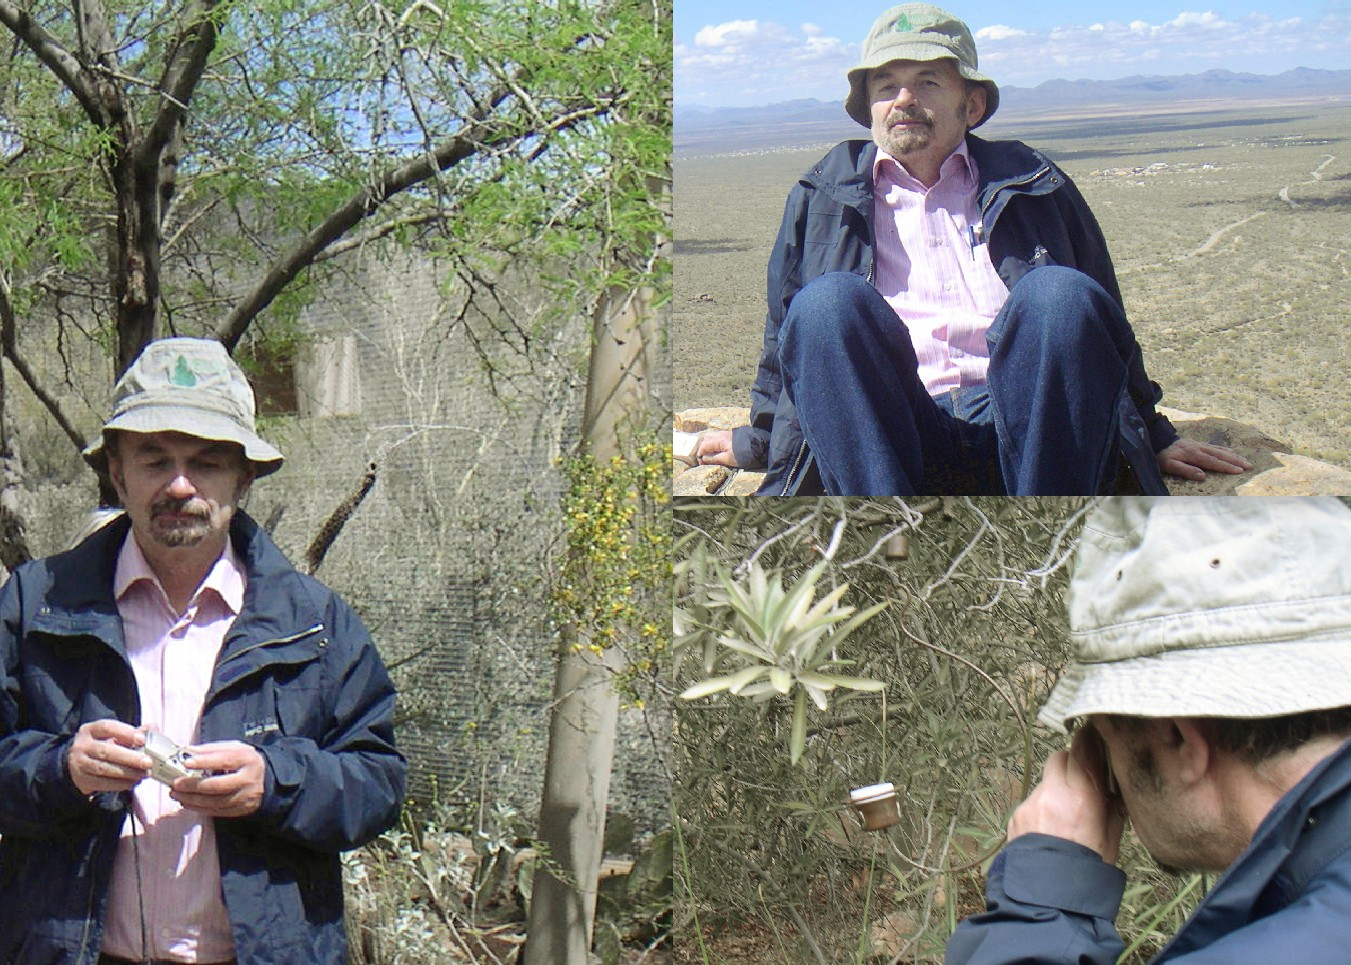
\includegraphics[width=0.95\columnwidth]{07March24HaraldCollageDesertMuseum.jpg}}
\caption{Harald Fritzsch visiting Arizona-Sonora Desert Museum in Spring 2007. Pictures and picture assembly by Johann Rafelski
}
\label{Fig:AZcolloq2007} 
\end{figure}

These meetings offered an opportunity to exchange ideas the  origin of neutrino mass and parameters of  the standard model were close to his heart. Were these parameters really natural constants on cosmological time scale? In Figure\,\ref{Fig:RANP2004} we see Harald's first transparency ``Time Dependence of QCD and Experimental Tests'' made at at the 9th Hadron Physics and 7th Relativistic Aspects of Nuclear Physics (HADRON-RANP 2004): A Joint Meeting on QCD and QGP: Rio de Janeiro, Brazil, March 28-April 3, 2004~\cite{Fritzsch:2004civ}, a meeting we both attended. We see that Harald modified slightly by hand the typed transparency to introduce the meeting specific context in a talk which arose from another publication of the epoch, Ref.\,\cite{Calmet:2001nu}. 

\begin{figure}%[ht]
\centerline{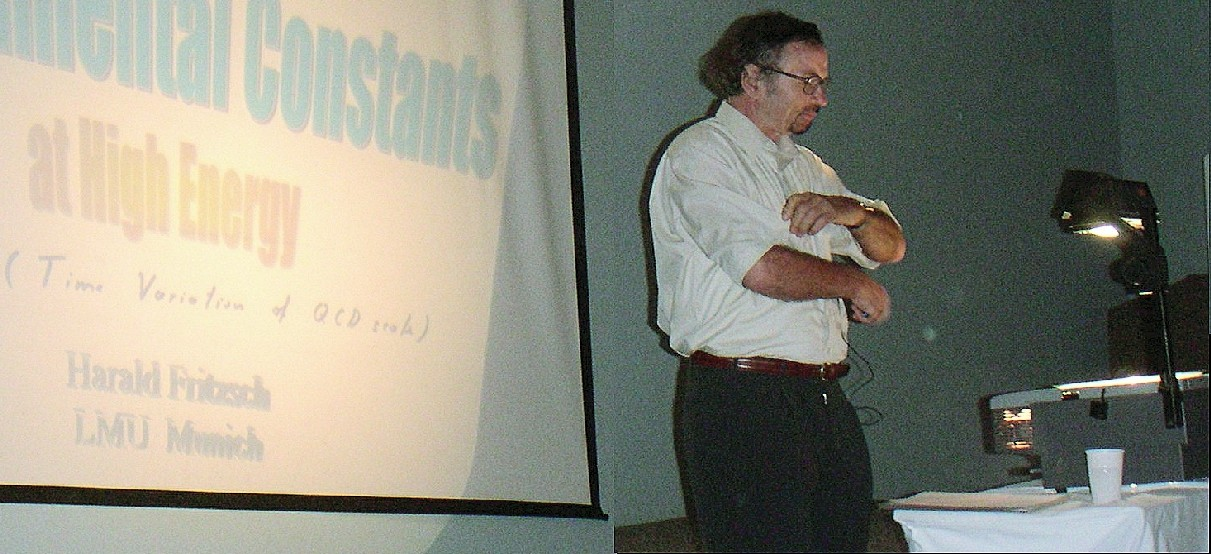
\includegraphics[width=0.95\columnwidth]{04RANPHarald1Ed.jpg}}
\caption{Harald begins his presentation in Rio de Janeiro 2004 about time dependence of QCD, see text for details. Picture by Johann Rafelski
}
\label{Fig:RANP2004} 
\end{figure}
 
%%%%%%%%%%%%%%%%%%%%%%%%%%%%%%%%%%%%


\bibliographystyle{ws-rv-van}
\bibliography{Rafelski_Steinmetz_for_Harald}
%%%%%%%%%%%%%%%%%%%%%%%%%%%%%%%%%%%%
\end{document} 
%%%%%%%%%%%%%%%%%%%%%%%%%%%%%%%%%%%%
